% !TeX program = xelatex
\documentclass[12pt,a4paper,oneside]{report}

% --------------------------------------------------------------------------
% Báo cáo kỹ thuật Hand Gesture Air Drawing System
% Biên dịch từ thư mục gốc dự án:
%   xelatex Bao_cao_Hand_Gesture_Air_Drawing.tex
%   xelatex Bao_cao_Hand_Gesture_Air_Drawing.tex
% --------------------------------------------------------------------------

\usepackage[a4paper,top=22mm,bottom=24mm,left=24mm,right=20mm,headheight=16pt]{geometry}
\usepackage{fontspec}
\defaultfontfeatures{Ligatures=TeX,Scale=MatchLowercase}
\IfFontExistsTF{Times New Roman}
  {\setmainfont{Times New Roman}}
  {\setmainfont{TeX Gyre Termes}}
\IfFontExistsTF{Be Vietnam Pro}
  {\setsansfont{Be Vietnam Pro}}
  {\IfFontExistsTF{Arial}
    {\setsansfont{Arial}}
    {\setsansfont{TeX Gyre Heros}}}
\IfFontExistsTF{Cascadia Mono}
  {\setmonofont{Cascadia Mono}}
  {\setmonofont{TeX Gyre Cursor}}

\XeTeXlinebreaklocale "vi"
\XeTeXlinebreakskip = 0pt plus 1pt

\usepackage{microtype}
\usepackage{setspace}
\usepackage{graphicx}
\usepackage{booktabs}
\usepackage{tabularx}
\usepackage{longtable}
\usepackage{array}
\usepackage{multirow}
\usepackage{enumitem}
\usepackage{amsmath,amssymb}
\usepackage{tikz}
\usetikzlibrary{arrows.meta,positioning,shapes.geometric,calc,fit,backgrounds}
\usepackage[most]{tcolorbox}
\usepackage{titlesec}
\usepackage{fancyhdr}
\usepackage{caption}
\usepackage{float}
\usepackage{hyperref}

% --------------------------------------------------------------------------
% Hệ màu xanh lá -- đỏ
% --------------------------------------------------------------------------
\definecolor{Forest}{HTML}{0B5D3B}
\definecolor{Leaf}{HTML}{238636}
\definecolor{Mint}{HTML}{EAF7EF}
\definecolor{MintDark}{HTML}{B8E0C4}
\definecolor{SignalRed}{HTML}{B4232A}
\definecolor{Coral}{HTML}{E45756}
\definecolor{Rose}{HTML}{FCEDEE}
\definecolor{Ink}{HTML}{17211D}
\definecolor{Slate}{HTML}{53635B}
\definecolor{Paper}{HTML}{FBFDFB}
\definecolor{Line}{HTML}{D8E4DC}
\definecolor{Gold}{HTML}{C98B21}

\hypersetup{
  colorlinks=true,
  linkcolor=Forest,
  urlcolor=SignalRed,
  citecolor=Forest,
  pdfauthor={Nhóm phát triển Hand Gesture Air Drawing System},
  pdftitle={Báo cáo kỹ thuật sản phẩm Hand Gesture Air Drawing System},
  pdfsubject={Computer Vision, MediaPipe, OpenCV, tương tác cử chỉ tay}
}

\setstretch{1.16}
\setlength{\parindent}{0pt}
\setlength{\parskip}{5pt}
\setlist[itemize]{leftmargin=6mm,itemsep=2pt,topsep=3pt}
\setlist[enumerate]{leftmargin=7mm,itemsep=2pt,topsep=3pt}
\setlength{\tabcolsep}{5pt}
\renewcommand{\arraystretch}{1.18}
\graphicspath{{demo/}}

\newcolumntype{Y}{>{\raggedright\arraybackslash}X}
\newcolumntype{L}[1]{>{\raggedright\arraybackslash}p{#1}}
\newcolumntype{C}[1]{>{\centering\arraybackslash}p{#1}}

\titleformat{\chapter}[display]
  {\sffamily\bfseries\color{Forest}}
  {\filleft\color{SignalRed}\fontsize{42}{42}\selectfont\thechapter}
  {-5pt}
  {\titlerule[1.2pt]\vspace{7pt}\Huge}
  [\vspace{3pt}{\color{SignalRed}\titlerule[0.6pt]}]
\titlespacing*{\chapter}{0pt}{-15pt}{20pt}
\titleformat{\section}
  {\Large\sffamily\bfseries\color{Forest}}
  {\thesection}{0.7em}{}
\titleformat{\subsection}
  {\large\sffamily\bfseries\color{SignalRed}}
  {\thesubsection}{0.7em}{}

\pagestyle{fancy}
\fancyhf{}
\fancyhead[L]{\sffamily\small\color{Forest}HAND GESTURE AIR DRAWING SYSTEM}
\fancyhead[R]{\sffamily\small\color{SignalRed}\leftmark}
\fancyfoot[L]{\sffamily\footnotesize\color{Slate}Tài liệu kỹ thuật sản phẩm Computer Vision}
\fancyfoot[R]{\sffamily\bfseries\color{Forest}\thepage}
\renewcommand{\headrulewidth}{0.5pt}
\renewcommand{\footrulewidth}{0.4pt}
\renewcommand{\headrule}{\hbox to\headwidth{\color{Forest}\leaders\hrule height \headrulewidth\hfill}}
\renewcommand{\footrule}{\hbox to\headwidth{\color{SignalRed}\leaders\hrule height \footrulewidth\hfill}}

\captionsetup{
  font=small,
  labelfont={bf,color=Forest},
  textfont={color=Ink},
  justification=centering
}
\renewcommand{\contentsname}{Mục lục}
\renewcommand{\figurename}{Hình}
\renewcommand{\tablename}{Bảng}
\renewcommand{\chaptername}{Chương}
\renewcommand{\bibname}{Tài liệu tham khảo}

\newtcolorbox{greenbox}[1][]{
  enhanced,
  breakable,
  colback=Mint,
  colframe=Forest,
  coltitle=white,
  fonttitle=\sffamily\bfseries,
  boxrule=0.7pt,
  arc=2mm,
  left=4mm,right=4mm,top=3mm,bottom=3mm,
  title=#1
}
\newtcolorbox{redbox}[1][]{
  enhanced,
  breakable,
  colback=Rose,
  colframe=SignalRed,
  coltitle=white,
  fonttitle=\sffamily\bfseries,
  boxrule=0.7pt,
  arc=2mm,
  left=4mm,right=4mm,top=3mm,bottom=3mm,
  title=#1
}
\newtcolorbox{metricbox}[1][]{
  enhanced,
  colback=Paper,
  colframe=Line,
  borderline west={3pt}{0pt}{Leaf},
  boxrule=0.5pt,
  arc=1mm,
  left=4mm,right=4mm,top=3mm,bottom=3mm,
  title=#1,
  coltitle=Forest,
  fonttitle=\sffamily\bfseries
}
\newtcolorbox{commandbox}{
  enhanced,
  colback=Ink,
  colframe=Forest,
  coltext=white,
  boxrule=0pt,
  arc=1.5mm,
  left=4mm,right=4mm,top=3mm,bottom=3mm,
  fontupper=\ttfamily\small
}

\newcommand{\status}[2]{%
  \tikz[baseline=(status.base)]\node[
    rounded corners=1.5mm,
    inner xsep=2.2mm,
    inner ysep=0.7mm,
    fill=#1!12,
    text=#1,
    font=\sffamily\bfseries\footnotesize
  ] (status) {#2};%
}
\newcommand{\safeimage}[2][]{%
  \IfFileExists{#2}
    {\includegraphics[#1]{#2}}
    {\fbox{\parbox[c][45mm][c]{0.9\linewidth}{\centering
      \sffamily\color{Slate}Không tìm thấy ảnh: \texttt{#2}}}}%
}
\newcommand{\codepath}[1]{\texttt{\detokenize{#1}}}

\begin{document}
\color{Ink}

% --------------------------------------------------------------------------
% Trang bìa
% --------------------------------------------------------------------------
\begin{titlepage}

\begin{tikzpicture}[remember picture,overlay]
  \fill[Paper] (current page.south west) rectangle (current page.north east);
  \fill[Forest] (current page.north west)
    rectangle ([yshift=-63mm]current page.north east);
  \fill[SignalRed]
    ([xshift=-17mm]current page.north east)
    -- (current page.north east)
    -- ([yshift=-118mm]current page.north east)
    -- ([xshift=-39mm,yshift=-76mm]current page.north east)
    -- cycle;
  \fill[Leaf!70]
    ([yshift=18mm]current page.south west)
    rectangle ([yshift=23mm]current page.south east);
  \fill[SignalRed]
    ([yshift=12mm]current page.south west)
    rectangle ([yshift=18mm]current page.south east);
  \draw[white,opacity=.16,line width=1pt]
    ([xshift=15mm,yshift=-15mm]current page.north west)
    grid[xstep=10mm,ystep=10mm]
    ([xshift=-15mm,yshift=-58mm]current page.north east);
  \foreach \x/\y in {30/-28,47/-19,64/-33,80/-23,96/-39,112/-25,128/-35,145/-20}{
    \fill[white,opacity=.68] ([xshift=\x mm,yshift=\y mm]current page.north west)
      circle (1.7mm);
  }
\end{tikzpicture}

\vspace*{8mm}
{\sffamily\bfseries\color{white}\fontsize{15}{18}\selectfont
TÀI LIỆU PHÂN TÍCH \& THIẾT KẾ SẢN PHẨM}

\vspace{36mm}
{\sffamily\bfseries\color{Forest}\fontsize{31}{36}\selectfont
HAND GESTURE\\[2mm]AIR DRAWING SYSTEM\par}
\vspace{5mm}
{\sffamily\color{SignalRed}\fontsize{18}{23}\selectfont
Nền tảng tương tác thị giác máy tính\\
bằng cử chỉ tay thời gian thực\par}

\vspace{12mm}
\begin{tcolorbox}[
  enhanced,
  width=\textwidth,
  colback=white,
  colframe=Line,
  borderline west={4pt}{0pt}{Forest},
  borderline east={4pt}{0pt}{SignalRed},
  boxrule=.5pt,
  arc=2mm,
  left=6mm,right=6mm,top=5mm,bottom=5mm
]
\sffamily
\begin{tabularx}{\linewidth}{L{35mm}Y}
\textbf{\color{Forest}Phiên bản sản phẩm} & 1.0.0\\
\textbf{\color{Forest}Nền tảng} & Windows 10/11, Python 3.14 (64-bit)\\
\textbf{\color{Forest}Lĩnh vực} & Computer Vision, Human--Computer Interaction, Gesture Recognition\\
\textbf{\color{Forest}Phạm vi tài liệu} & Kiến trúc, pipeline xử lý ảnh, thuật toán cử chỉ, nhận dạng ký tự, kiểm thử, quyền riêng tư và lộ trình sản phẩm\\
\end{tabularx}
\end{tcolorbox}

\vfill
{\sffamily\color{Slate}
\textbf{Ngày cập nhật:} 27 tháng 7 năm 2026\par
\textbf{Nguồn phân tích:} mã nguồn, cấu hình và bộ kiểm thử trong kho dự án\par}
\end{titlepage}

\pagenumbering{roman}
\tableofcontents
\clearpage

\chapter*{Tóm tắt điều hành}
\addcontentsline{toc}{chapter}{Tóm tắt điều hành}
\markboth{Tóm tắt điều hành}{Tóm tắt điều hành}

\begin{greenbox}[Giá trị cốt lõi]
Hand Gesture Air Drawing System (tên gói: \textbf{AirGesture Studio}) biến webcam phổ thông thành một bề mặt tương tác không chạm. Người dùng có thể vẽ bằng đầu ngón tay, điều khiển thanh công cụ bằng cử chỉ, nhận dạng nét viết thành ký tự sạch, hoặc chụp ảnh và giải trò chơi ghép hình bằng thao tác chụm--thả.
\end{greenbox}

Sản phẩm được xây dựng theo hướng \textit{local-first}: khung hình camera và landmarks bàn tay được xử lý trên máy bằng OpenCV và MediaPipe Tasks. Luồng theo dõi sử dụng 21 mốc trên mỗi bàn tay, bộ lọc One Euro cho toàn bộ landmarks, làm mượt thích ứng theo vận tốc cho nét vẽ, cùng cơ chế hysteresis để chống rung trạng thái pinch.

\begin{table}[H]
\centering
\caption{Ảnh chụp nhanh trạng thái sản phẩm}
\begin{tabularx}{\textwidth}{L{40mm}Y}
\toprule
\textbf{Hạng mục} & \textbf{Trạng thái hiện tại}\\
\midrule
Luồng sản phẩm & Menu chính, Air Drawing, Camera Check, Gesture Puzzle\\
Đầu vào thị giác & Webcam 1280$\times$720, 30 FPS theo cấu hình mặc định, ảnh mirror\\
Nhận diện tay & MediaPipe Hand Landmarker, tối đa 1 tay khi vẽ và 2 tay khi puzzle\\
Nhận dạng ký tự & Template một nét A--Z và 0--9; sẵn giao diện tích hợp ONNX tùy chọn\\
Độ bền runtime & Camera backend fallback, retry khung hình, reconnect có giới hạn, lỗi có hướng dẫn\\
Quyền riêng tư & Xin đồng ý trước khi khởi tạo MediaPipe; xử lý camera cục bộ\\
Chất lượng phần mềm & \textbf{78/78} kiểm thử tự động đạt tại thời điểm lập báo cáo\\
\bottomrule
\end{tabularx}
\end{table}

\begin{redbox}[Kết luận sản phẩm]
Đây là một prototype sản phẩm Computer Vision có cấu trúc tốt và đã vượt qua giai đoạn ``demo thuật toán'' đơn thuần: có quản lý cấu hình, quyền riêng tư, dữ liệu runtime, xử lý lỗi, giao diện responsive và kiểm thử hồi quy. Khoảng trống lớn nhất trước khi đánh giá ở quy mô thương mại là thiếu bộ dữ liệu thực nghiệm có nhãn, benchmark độ chính xác/độ trễ trên nhiều thiết bị, và model ONNX chữ viết tay được huấn luyện--đóng gói chính thức.
\end{redbox}

\clearpage
\pagenumbering{arabic}

% --------------------------------------------------------------------------
\chapter{Tổng quan sản phẩm}

\section{Bài toán và mục tiêu}

Các giao diện chuột, bàn phím hoặc màn hình cảm ứng không phù hợp với mọi bối cảnh. Trong lớp học, thuyết trình, kiosk, trò chơi vận động nhẹ hoặc môi trường cần hạn chế tiếp xúc bề mặt, cử chỉ tay trước camera tạo ra một kênh tương tác tự nhiên và chi phí thấp.

Mục tiêu của dự án là xây dựng một ứng dụng desktop:

\begin{itemize}
  \item vận hành với webcam phổ thông, không cần găng tay hay cảm biến chiều sâu;
  \item phản hồi thời gian thực và giữ nét vẽ ổn định trước nhiễu landmark;
  \item cung cấp hai trải nghiệm có giá trị rõ ràng: sáng tạo bằng nét vẽ và trò chơi ghép hình;
  \item xử lý dữ liệu camera cục bộ, có thông báo đồng ý và vị trí lưu dữ liệu minh bạch;
  \item chịu được các sự cố thực tế như camera bận, mất frame hoặc thiết bị ngắt kết nối.
\end{itemize}

\section{Phạm vi tính năng}

\begin{table}[H]
\centering
\caption{Các capability chính của AirGesture Studio}
\begin{tabularx}{\textwidth}{L{35mm}L{43mm}Y}
\toprule
\textbf{Capability} & \textbf{Đầu vào} & \textbf{Đầu ra / giá trị}\\
\midrule
Air Drawing & Một tay; pinch ngón cái--trỏ; tư thế hai ngón & Nét vẽ màu, tẩy, đổi cỡ bút, undo, clear, lưu PNG\\
Nhận dạng ký tự & Một stroke sau khi người dùng nhả pinch & Ký tự sạch A--Z/0--9 nếu đủ tin cậy; tối đa 3 gợi ý nếu mơ hồ\\
Gesture Puzzle & Cử chỉ khung hình bằng hai tay; pinch chọn ô & Puzzle 3$\times$3 hoặc 4$\times$4, đếm thời gian và số lượt\\
Camera Check & Khung hình, độ sáng, số tay theo dõi được & Phản hồi framing, ánh sáng, camera index/backend/resolution/FPS\\
Quản lý camera & Phím A/D/R và cơ chế dò thiết bị & Chọn camera trong phiên, quét lại và fallback backend trên Windows\\
\bottomrule
\end{tabularx}
\end{table}

\section{Người dùng và kịch bản sử dụng}

\begin{itemize}
  \item \textbf{Giáo viên / người thuyết trình:} minh họa nhanh trước webcam mà không chạm màn hình.
  \item \textbf{Học sinh:} luyện phối hợp tay--mắt, vẽ ký tự đơn và nhận phản hồi trực quan.
  \item \textbf{Người dùng giải trí:} tạo puzzle từ chính khung hình camera và chơi bằng pinch.
  \item \textbf{Nhà phát triển / nghiên cứu HCI:} dùng cấu trúc module làm nền cho thử nghiệm gesture, smoothing và recognition.
\end{itemize}

\section{Giao diện hiện tại}

\begin{figure}[H]
\centering
\safeimage[width=.88\textwidth]{demo/airgesture-studio.png}
\caption{Menu chính AirGesture Studio với lựa chọn chế độ và camera}
\end{figure}

\begin{figure}[H]
\centering
\begin{minipage}[t]{.49\textwidth}
  \centering
  \safeimage[width=\linewidth]{demo/air-drawing.png}
  \caption*{\textbf{(a)} Air Drawing và thanh công cụ cử chỉ}
\end{minipage}\hfill
\begin{minipage}[t]{.49\textwidth}
  \centering
  \safeimage[width=\linewidth]{demo/camera-check.png}
  \caption*{\textbf{(b)} Camera Check và chẩn đoán đầu vào}
\end{minipage}
\caption{Hai màn hình hỗ trợ tương tác và chuẩn bị môi trường}
\end{figure}

% --------------------------------------------------------------------------
\chapter{Kiến trúc hệ thống}

\section{Kiến trúc logic}

\begin{figure}[H]
\centering
\resizebox{\textwidth}{!}{%
\begin{tikzpicture}[
  node distance=10mm and 11mm,
  block/.style={
    draw=Forest,
    fill=Mint,
    rounded corners=2mm,
    minimum width=31mm,
    minimum height=12mm,
    align=center,
    font=\sffamily\small\bfseries
  },
  redblock/.style={
    block,
    draw=SignalRed,
    fill=Rose
  },
  arrow/.style={-{Latex[length=2.6mm]},thick,color=Slate}
]
\node[block] (camera) {Webcam\\OpenCV};
\node[block,right=of camera] (capture) {Capture, mirror\\fallback, reconnect};
\node[block,right=of capture] (mp) {MediaPipe Tasks\\21 landmarks/tay};
\node[block,right=of mp] (filter) {One Euro filter\\+ dropout tolerance};

\node[redblock,below=14mm of mp] (gesture) {Diễn giải cử chỉ\\pinch / finger state};
\node[block,below left=14mm and 13mm of gesture] (drawing) {Air Drawing\\canvas + toolbar};
\node[block,below=14mm of gesture] (recognition) {Recognition\\template + ONNX};
\node[redblock,below right=14mm and 13mm of gesture] (puzzle) {Gesture Puzzle\\state machine};

\node[block,below=16mm of recognition] (ui) {HUD / responsive window\\thông báo và lưu kết quả};

\draw[arrow] (camera) -- (capture);
\draw[arrow] (capture) -- (mp);
\draw[arrow] (mp) -- (filter);
\draw[arrow] (filter) |- (gesture);
\draw[arrow] (gesture) -- (drawing);
\draw[arrow] (gesture) -- (recognition);
\draw[arrow] (gesture) -- (puzzle);
\draw[arrow] (drawing) |- (ui);
\draw[arrow] (recognition) -- (ui);
\draw[arrow] (puzzle) |- (ui);
\end{tikzpicture}}
\caption{Luồng dữ liệu chính từ camera đến trải nghiệm người dùng}
\end{figure}

\section{Phân rã module}

\begin{longtable}{L{32mm}L{40mm}L{64mm}}
\caption{Trách nhiệm của các module quan trọng}\\
\toprule
\textbf{Nhóm} & \textbf{Tệp tiêu biểu} & \textbf{Trách nhiệm}\\
\midrule
\endfirsthead
\toprule
\textbf{Nhóm} & \textbf{Tệp tiêu biểu} & \textbf{Trách nhiệm}\\
\midrule
\endhead
\codepath{core/} & \codepath{camera.py} & Khám phá camera, lựa chọn backend, cấu hình capture, đọc frame, retry và reconnect.\\
& \codepath{hand_tracker.py} & Nạp MediaPipe theo nhu cầu, kiểm tra SHA-256 model, detect video, lọc 21 landmarks, quy đổi pixel.\\
& \codepath{smoothing.py} & EMA, smoothing thích ứng theo vận tốc và One Euro filter 3D.\\
\midrule
\codepath{drawing/} & \codepath{main.py} & Vòng lặp Air Drawing, trạng thái stroke, pinch, toolbar, nhận dạng và hiển thị.\\
& \codepath{canvas.py} & Layer nét vẽ, tẩy, lịch sử undo, compositing và lưu ảnh nguyên tử.\\
& \codepath{letter_recognizer.py} & Làm sạch, chuẩn hóa, resample stroke; template matching; fusion ONNX; confidence gate.\\
& \codepath{toolbar.py} & Hit-test, dwell/select và bố cục toolbar responsive.\\
\midrule
\codepath{puzzle/} & \codepath{capture_gesture.py} & Cử chỉ chụp hai tay qua các pha waiting/center/spread/hold.\\
& \codepath{gesture.py} & Pinch hysteresis và dung sai mất landmark ngắn.\\
& \codepath{board.py} & Cắt ảnh vuông, tạo tile, shuffle, swap, render, kiểm tra hoàn thành.\\
& \codepath{main.py} & State machine capture--countdown--playing--victory.\\
\midrule
\codepath{config/} & \codepath{settings.py} & Nạp JSON, ánh xạ dataclass, kiểm tra trường lạ và miền giá trị.\\
\codepath{ui/} & \codepath{window.py}, \codepath{runtime_errors.py} & Cửa sổ responsive/fullscreen, đóng native, dialog lỗi và cleanup.\\
\bottomrule
\end{longtable}

\section{Nguyên tắc thiết kế}

\begin{metricbox}[Separation of concerns]
Camera, hand tracking, smoothing, gesture, canvas, recognition và HUD được tách thành module riêng. Điều này cho phép kiểm thử thuật toán mà không cần camera vật lý và giảm ảnh hưởng dây chuyền khi tinh chỉnh một ngưỡng.
\end{metricbox}

\begin{metricbox}[Config-driven]
Các ngưỡng nhạy cảm với thiết bị và người dùng nằm trong JSON cấu hình. Cấu hình mặc định được sao chép sang vùng dữ liệu người dùng ở lần chạy đầu, tránh ghi ngược vào thư mục cài đặt.
\end{metricbox}

\begin{metricbox}[Fail safely]
Các lỗi camera, model, cấu hình và OpenCV được chuyển thành thông báo có hành động khắc phục. Camera và cửa sổ được giải phóng trong khối cleanup kể cả khi có ngoại lệ.
\end{metricbox}

% --------------------------------------------------------------------------
\chapter{Pipeline Computer Vision}

\section{Thu nhận và chuẩn hóa khung hình}

Camera mặc định yêu cầu 1280$\times$720 tại 30 FPS, buffer size bằng 1 để giảm độ trễ. Trên Windows, ứng dụng lần lượt thử:

\begin{center}
\status{Forest}{DirectShow}
\quad$\longrightarrow$\quad
\status{Forest}{Media Foundation}
\quad$\longrightarrow$\quad
\status{SignalRed}{OpenCV Default}
\end{center}

Sau khi đọc, frame được lật ngang khi \codepath{mirror=true}, tạo cảm giác tương tác như gương. Trong tracker, ảnh BGR của OpenCV được chuyển sang RGB trước khi đóng gói thành \codepath{mp.Image}.

Mỗi frame ở chế độ MediaPipe \codepath{VIDEO} đi kèm timestamp tăng đơn điệu. Nếu đồng hồ đo cho giá trị không tăng, mã nguồn ép timestamp mới lớn hơn timestamp trước ít nhất 1 ms, tránh vi phạm hợp đồng của MediaPipe.

\section{Phát hiện bàn tay và 21 landmarks}

MediaPipe Hand Landmarker trả về 21 điểm chuẩn hóa $(x,y,z)$ cho mỗi bàn tay cùng handedness. Ứng dụng dùng:

\begin{itemize}
  \item tối đa \textbf{1 tay} trong Air Drawing;
  \item tối đa \textbf{2 tay} trong Gesture Puzzle;
  \item các điểm quan trọng: thumb tip (4), index tip (8), các tip/PIP của ngón giữa, áp út và út;
  \item tọa độ chuẩn hóa được kẹp vào miền ảnh trước khi đổi sang pixel.
\end{itemize}

Model \codepath{hand_landmarker.task} được đóng gói cục bộ. Trước khi khởi tạo, chương trình tính SHA-256 và so sánh với digest kỳ vọng đối với model bundled. Kiểm tra này phát hiện model bị hỏng hoặc bị thay đổi ngoài ý muốn.

\section{Lọc One Euro cho landmark}

Từng landmark 3D có một bộ lọc riêng. Với khoảng thời gian $\Delta t$, hệ số low-pass cho tần số cắt $f_c$ là:

\begin{equation}
  \alpha(f_c,\Delta t)=
  \frac{1}{1+\dfrac{1}{2\pi f_c\Delta t}}.
\end{equation}

Đạo hàm vị trí được lọc trước để ước lượng tốc độ $v_t$. Tần số cắt động:

\begin{equation}
  f_{c,t}=f_{\min}+\beta\lVert v_t\rVert.
\end{equation}

Khi tay gần đứng yên, $f_c$ thấp giúp giảm jitter. Khi tay di chuyển nhanh, $f_c$ tăng để giảm độ trễ. Ngoài ra, dịch chuyển XY trong một frame bị giới hạn bởi \codepath{max_jump}; đây là lớp bảo vệ trước outlier đơn lẻ.

\begin{table}[H]
\centering
\caption{Profile One Euro mặc định theo chế độ}
\begin{tabularx}{\textwidth}{L{30mm}C{18mm}C{18mm}C{24mm}C{20mm}}
\toprule
\textbf{Chế độ} & $f_{\min}$ & $\beta$ & Derivative cutoff & Max jump\\
\midrule
Air Drawing & 1.35 & 0.45 & 1.0 & 0.18\\
Gesture Puzzle & 1.65 & 0.55 & 1.0 & 0.22\\
Camera Check & 1.50 & 0.45 & 1.0 & 0.22\\
\bottomrule
\end{tabularx}
\end{table}

Nếu không phát hiện tay quá số frame cho phép, bank bộ lọc được xóa để bàn tay xuất hiện lại không bị kéo về vị trí cũ.

\section{Làm mượt thích ứng cho nét vẽ}

Sau lọc landmark, index tip trong Air Drawing còn đi qua một tầng smoothing theo vận tốc. Vận tốc tức thời:

\begin{equation}
  s_t=\frac{\lVert r_t-r_{t-1}\rVert}{\Delta t},
\end{equation}

với $r_t$ là điểm raw. Hệ số $\alpha_t$ nội suy giữa \codepath{slow_alpha=0.18} và \codepath{fast_alpha=0.82} bằng hàm smoothstep trong dải 90--950 pixel/s:

\begin{align}
  u &= \operatorname{clip}\left(\frac{s_t-s_{\mathrm{slow}}}
  {s_{\mathrm{fast}}-s_{\mathrm{slow}}},0,1\right),\\
  h(u) &= u^2(3-2u),\\
  p_t &= p_{t-1}+\alpha_t(r_t-p_{t-1}).
\end{align}

Chuyển động chậm được lọc mạnh để nét ổn định; chuyển động nhanh bám tay tốt hơn. Hệ thống phản ứng ngay khi tăng tốc nhưng giảm tốc êm với \codepath{speed_smoothing_alpha=0.35}. Hai frame mất detection ngắn vẫn giữ điểm cuối, hạn chế stroke bị đứt.

\section{Nhận biết pinch bằng hysteresis}

Khoảng cách Euclid giữa thumb tip và index tip:

\begin{equation}
  d_t=\sqrt{(x_{\mathrm{thumb}}-x_{\mathrm{index}})^2+
  (y_{\mathrm{thumb}}-y_{\mathrm{index}})^2}.
\end{equation}

Trạng thái chỉ bật khi $d_t\le T_{\mathrm{pinch}}$ và chỉ tắt khi
$d_t\ge T_{\mathrm{release}}$, với $T_{\mathrm{release}}>T_{\mathrm{pinch}}$.
Khoảng chết giữa hai ngưỡng ngăn trạng thái dao động khi ngón tay ở sát biên.

\begin{table}[H]
\centering
\caption{Ngưỡng pinch mặc định theo luồng}
\begin{tabular}{lccc}
\toprule
\textbf{Luồng} & $T_{\mathrm{pinch}}$ & $T_{\mathrm{release}}$ & Dung sai mất frame\\
\midrule
Air Drawing & 46 px & 68 px & 2 frame\\
Gesture Puzzle & 48 px & 72 px & 2 frame\\
\bottomrule
\end{tabular}
\end{table}

\begin{redbox}[Lưu ý hiệu chuẩn]
Ngưỡng tính theo pixel nên phụ thuộc khoảng cách từ tay đến camera, tiêu cự và độ phân giải thực tế. Cấu hình hiện tại phù hợp cho prototype 720p nhưng nên chuẩn hóa theo kích thước bàn tay hoặc khoảng cách landmark để tăng khả năng chuyển thiết bị.
\end{redbox}

% --------------------------------------------------------------------------
\chapter{Air Drawing và nhận dạng ký tự}

\section{Luồng điều khiển}

\begin{enumerate}
  \item Người dùng đưa tay vào vùng quan sát; MediaPipe trả về landmarks đã lọc.
  \item Pinch ngón cái--trỏ bắt đầu hoặc tiếp tục stroke. Index tip đã làm mượt là đầu bút.
  \item Nếu khoảng cách giữa hai điểm stroke liên tiếp không vượt 180 px, canvas nối chúng; bước nhảy lớn kết thúc stroke cũ thay vì vẽ một đường dài sai.
  \item Khi nhả pinch, debouncer chờ 0.18 giây và có grace 4 frame để tránh kết thúc sớm do tracking chập chờn.
  \item Stroke được làm sạch, nhận dạng và commit vào layer chính. Nếu đủ tin cậy, hệ thống snap thành ký tự sạch.
  \item Tư thế giơ ngón trỏ và ngón giữa được dùng để di chuyển con trỏ, hover/chọn công cụ mà không vẽ.
\end{enumerate}

\section{Canvas và công cụ}

Canvas ảo tách khỏi frame camera, nhờ đó nét có thể được compositing lên preview mà không sửa ảnh nguồn. Các công cụ gồm năm màu đỏ, xanh lá, xanh dương, vàng, trắng; tẩy; bút mảnh/dày; clear; save; mở thư mục; undo.

\begin{table}[H]
\centering
\caption{Thông số vẽ mặc định}
\begin{tabularx}{\textwidth}{L{52mm}L{30mm}Y}
\toprule
\textbf{Thông số} & \textbf{Giá trị} & \textbf{Ý nghĩa}\\
\midrule
Default / thin / thick brush & 10 / 7 / 16 px & Cỡ bút ban đầu và hai preset toolbar\\
Eraser size & 34 px & Vùng xóa rộng hơn nét bút để thao tác dễ\\
Maximum bridge distance & 180 px & Không nối stroke qua bước nhảy tracking quá lớn\\
Undo depth & 20 hành động & Lưu snapshot trước stroke vẽ hoặc tẩy\\
Recognition display & 2.5 s & Thời gian hiển thị phát hiện/gợi ý\\
\bottomrule
\end{tabularx}
\end{table}

Lưu ảnh được thực hiện theo hướng nguyên tử: encode và ghi tệp tạm trước, sau đó thay tên. Tên có timestamp đến microsecond và suffix duy nhất nếu trùng, vì vậy không âm thầm ghi đè kết quả cũ.

\section{Pipeline nhận dạng một stroke}

\begin{figure}[H]
\centering
\begin{tikzpicture}[
  node distance=7mm,
  step/.style={
    draw=Forest,
    fill=Mint,
    rounded corners=1.5mm,
    minimum height=10mm,
    text width=27mm,
    align=center,
    font=\sffamily\small
  },
  decision/.style={
    draw=SignalRed,
    fill=Rose,
    diamond,
    aspect=2.0,
    align=center,
    font=\sffamily\scriptsize
  },
  arrow/.style={-{Latex[length=2.2mm]},thick,color=Slate}
]
\node[step] (raw) {Stroke raw};
\node[step,right=of raw] (clean) {Lọc điểm gần nhau, làm mượt};
\node[step,right=of clean] (norm) {Chuẩn hóa và resample 64 điểm};
\node[step,right=of norm] (match) {Template distance A--Z, 0--9};
\node[step,below=10mm of match] (onnx) {ONNX 1$\times$1$\times$64$\times$64 (tùy chọn)};
\node[decision,left=12mm of onnx] (gate) {Confidence\\và margin?};
\node[step,left=of gate,draw=SignalRed,fill=Rose] (result) {Snap ký tự\\hoặc gợi ý Top-3};
\draw[arrow] (raw) -- (clean);
\draw[arrow] (clean) -- (norm);
\draw[arrow] (norm) -- (match);
\draw[arrow] (match) -- (onnx);
\draw[arrow] (onnx) -- (gate);
\draw[arrow] (gate) -- (result);
\end{tikzpicture}
\caption{Pipeline nhận dạng ký tự một nét}
\end{figure}

\subsection{Template matching}

Các điểm sau làm sạch được chuẩn hóa theo vị trí và tỷ lệ, rồi resample thành 64 mẫu có khoảng cách dọc đường đi tương đối đồng đều. Mỗi ký tự có một hoặc nhiều template stroke. Khoảng cách đường đi nhỏ nhất giữa candidate và template được đổi thành confidence.

Hệ thống có xử lý riêng cho cặp \texttt{I}/\texttt{1} và đánh dấu các nhóm dễ nhầm:
\texttt{I--1}, \texttt{O--0}, \texttt{S--5}, \texttt{Z--2}, \texttt{B--8}, \texttt{G--6}.

\subsection{Confidence gate}

Candidate chỉ được snap khi:

\begin{itemize}
  \item confidence tốt nhất $\ge 0.74$;
  \item chênh lệch với hạng hai $\ge 0.07$;
  \item với cặp mơ hồ, margin yêu cầu tăng lên ít nhất $0.12$.
\end{itemize}

Nếu không qua gate nhưng confidence đủ 0.30, overlay hiển thị tối đa ba gợi ý. Thiết kế này ưu tiên \textbf{không tự sửa sai} hơn việc luôn ép stroke thành ký tự.

\subsection{Tích hợp ONNX tùy chọn}

Stroke được raster hóa thành ảnh grayscale 64$\times$64, padding 8 px, nét dày 4 px và chuẩn hóa vào tensor $1\times1\times64\times64$. Nếu model ONNX được cấu hình, điểm cuối:

\begin{equation}
  S(c)=(1-w)S_{\mathrm{template}}(c)+wS_{\mathrm{ONNX}}(c),
  \qquad w=0.70.
\end{equation}

Output mặc định phải có 36 score theo thứ tự A--Z rồi 0--9. Runtime OpenCV DNN tự áp dụng softmax nếu output chưa phải phân phối xác suất.

\begin{redbox}[Giới hạn hiện tại]
Kho mã nguồn chưa đóng gói một model ONNX chữ viết tay đã huấn luyện. Vì vậy chế độ mặc định là template recognition. Sản phẩm nhận dạng ký tự đơn, một stroke; chưa nhận dạng từ hoặc câu viết tay liên tục.
\end{redbox}

% --------------------------------------------------------------------------
\chapter{Gesture Puzzle}

\section{Cử chỉ chụp ảnh bằng hai tay}

Luồng capture theo bốn pha:

\begin{center}
\status{Slate}{WAITING}
\quad$\rightarrow$\quad
\status{Forest}{CENTER}
\quad$\rightarrow$\quad
\status{SignalRed}{SPREAD}
\quad$\rightarrow$\quad
\status{Forest}{HOLD / CAPTURE}
\end{center}

Hệ thống lấy thumb tip và index tip của mỗi tay, tổng cộng bốn điểm. Từ đó tính bounding box, tâm cụm, bán kính cụm và tỷ lệ spread. Capture tự động kích hoạt khi:

\begin{itemize}
  \item nhìn thấy đủ hai tay;
  \item độ mở đạt ít nhất 0.34 theo tỷ lệ chiều rộng/chiều cao frame;
  \item biến động tổng của $(x,y,w,h)$ không vượt ngưỡng động;
  \item trạng thái ổn định kéo dài ít nhất 5 frame.
\end{itemize}

Ngưỡng chuyển động động là giá trị lớn hơn giữa 64 px và 8\% cạnh ngắn frame. Người dùng luôn có phương án fallback bằng Space, Enter hoặc C.

\section{State machine trò chơi}

\begin{figure}[H]
\centering
\begin{tikzpicture}[
  state/.style={
    draw=Forest,
    very thick,
    fill=Mint,
    rounded corners=3mm,
    minimum width=34mm,
    minimum height=14mm,
    align=center,
    font=\sffamily\bfseries
  },
  redstate/.style={state,draw=SignalRed,fill=Rose},
  arrow/.style={-{Latex[length=2.5mm]},thick,color=Slate}
]
\node[state] (capture) {CAPTURE};
\node[state,right=18mm of capture] (countdown) {COUNTDOWN\\3 giây};
\node[redstate,right=18mm of countdown] (playing) {PLAYING};
\node[state,right=18mm of playing] (victory) {VICTORY};
\draw[arrow] (capture) -- node[above,font=\scriptsize\sffamily]{đủ gesture / phím} (countdown);
\draw[arrow] (countdown) -- node[above,font=\scriptsize\sffamily]{tạo board} (playing);
\draw[arrow] (playing) -- node[above,font=\scriptsize\sffamily]{đúng thứ tự} (victory);
\draw[arrow] (victory.south) to[bend left=30]
  node[below,font=\scriptsize\sffamily]{R: chơi lại} (capture.south);
\draw[arrow] (playing.south) to[bend right=30]
  node[below,font=\scriptsize\sffamily]{R: chụp lại} (capture.south);
\end{tikzpicture}
\caption{Máy trạng thái của Gesture Puzzle}
\end{figure}

Sau countdown, ảnh được crop/resize thành hình vuông, chia thành lưới 3$\times$3 hoặc 4$\times$4 rồi shuffle. Index tip điều khiển cursor; pinch bắt đầu trên một tile để chọn, nhả pinch trên tile khác để swap. Hệ thống tăng bộ đếm move khi swap hợp lệ và so sánh thứ tự tile với thứ tự đích để phát hiện victory.

\begin{figure}[H]
\centering
\begin{minipage}[t]{.49\textwidth}
  \centering
  \safeimage[width=\linewidth]{demo/gesture-puzzle-start.png}
  \caption*{\textbf{(a)} Pha chuẩn bị capture}
\end{minipage}\hfill
\begin{minipage}[t]{.49\textwidth}
  \centering
  \safeimage[width=\linewidth]{demo/gesture-puzzle-play.png}
  \caption*{\textbf{(b)} Pha chơi và điều khiển tile}
\end{minipage}
\caption{Trải nghiệm Gesture Puzzle}
\end{figure}

% --------------------------------------------------------------------------
\chapter{Trải nghiệm, độ tin cậy và an toàn}

\section{Thiết kế trải nghiệm}

Giao diện camera giữ tỷ lệ 16:9 và ánh xạ con trỏ theo vùng hiển thị thực tế, tránh sai lệch khi cửa sổ thay đổi kích thước hoặc frame bị crop. Cửa sổ hỗ trợ maximize, fullscreen bằng F11 và thoát fullscreen trước khi xử lý Esc như lệnh rời chế độ.

Camera Check là công cụ chẩn đoán chủ động, không phải bước bắt buộc trước mỗi trải nghiệm. Màn hình này báo:

\begin{itemize}
  \item số bàn tay hiện diện;
  \item mức sáng thấp/cao dựa trên ngưỡng 55--220;
  \item camera index, backend, độ phân giải nguồn và FPS driver;
  \item hướng dẫn cụ thể khi cần chỉnh ánh sáng hoặc vị trí tay.
\end{itemize}

\section{Khả năng chịu lỗi camera}

\begin{enumerate}
  \item Dò camera qua tối đa 5 index mặc định.
  \item Nếu mở thất bại, thử lần lượt các backend phù hợp Windows.
  \item Khi đọc frame lỗi, retry nhanh tối đa 2 lần.
  \item Nếu vẫn lỗi, giải phóng và mở lại camera tối đa 3 lần, nghỉ 0.20 giây giữa các lần.
  \item Nếu reconnect thành công, tiếp tục phiên và tăng bộ đếm reconnect.
  \item Nếu thất bại, hiển thị lỗi phân biệt ``không tìm thấy'', ``đã phát hiện nhưng không truy cập được'' và ``đã ngắt kết nối''.
\end{enumerate}

\section{Cấu hình an toàn}

JSON cấu hình được kiểm tra nghiêm ngặt: trường lạ, sai kiểu, giá trị ngoài miền và JSON hỏng đều bị từ chối với thông báo rõ. Điều này quan trọng với hệ CV vì ngưỡng không hợp lệ có thể làm gesture luôn bật, lọc mất ổn định hoặc camera không khởi tạo.

\section{Quyền riêng tư và bảo mật}

\begin{greenbox}[Local processing]
Khung hình camera và landmarks được xử lý cục bộ. Ứng dụng không có pipeline tải ảnh người dùng lên máy chủ. Ảnh chỉ được lưu khi người dùng chủ động bấm Save trong Air Drawing.
\end{greenbox}

Trước phiên hand tracking đầu tiên, ứng dụng hiển thị thông báo và yêu cầu đồng ý về operational metrics của MediaPipe. Lựa chọn mặc định là \textbf{No}; nếu từ chối, MediaPipe Task không được khởi tạo. Bản ghi đồng ý có version để chính sách cũ buộc xin lại consent khi cần.

Các lớp bảo vệ đáng chú ý:

\begin{itemize}
  \item lazy-load MediaPipe chỉ sau khi người dùng bắt đầu một chế độ tracking;
  \item kiểm tra SHA-256 model bundled;
  \item không lưu frame camera mặc định;
  \item đường dẫn dữ liệu user tách khỏi mã nguồn và thư mục cài đặt;
  \item log runtime xoay vòng, phục vụ chẩn đoán bản packaged không có terminal.
\end{itemize}

\begin{redbox}[Điểm cần hoàn tất trước phát hành công khai]
Mã nguồn hiện được đánh dấu all-rights-reserved. Cần chốt giấy phép nguồn mong muốn và hoàn tất hạng mục phê duyệt tái phân phối model được ghi trong \codepath{THIRD_PARTY_NOTICES.md}. Với triển khai offline nghiêm ngặt, cần kiểm chứng cấu hình metrics và network ở cấp hệ điều hành theo hướng dẫn trong \codepath{PRIVACY.md}.
\end{redbox}

% --------------------------------------------------------------------------
\chapter{Cấu hình và vận hành}

\section{Yêu cầu hệ thống}

\begin{table}[H]
\centering
\caption{Yêu cầu chạy ứng dụng}
\begin{tabularx}{\textwidth}{L{38mm}Y}
\toprule
\textbf{Thành phần} & \textbf{Yêu cầu}\\
\midrule
Hệ điều hành & Windows 10 hoặc Windows 11\\
Python & 3.14, kiến trúc 64-bit\\
Camera & Webcam hoạt động và được Windows cấp quyền truy cập\\
Runtime chính & MediaPipe 0.10.35; NumPy 2.5.0; OpenCV Contrib 4.13.0.92\\
Khuyến nghị hình ảnh & 1280$\times$720, 30 FPS, ánh sáng đều, bàn tay không bị che khuất\\
\bottomrule
\end{tabularx}
\end{table}

\section{Cài đặt và khởi chạy}

\begin{commandbox}
python --version\\
python -m venv .venv\\
.venv\textbackslash Scripts\textbackslash python.exe -m pip install --upgrade pip\\
.venv\textbackslash Scripts\textbackslash python.exe -m pip install -r requirements.txt\\[2mm]
.venv\textbackslash Scripts\textbackslash python.exe -m airgesture
\end{commandbox}

Các entry point trực tiếp:

\begin{commandbox}
.venv\textbackslash Scripts\textbackslash python.exe -m airgesture.drawing.main\\
.venv\textbackslash Scripts\textbackslash python.exe -m airgesture.puzzle.main
\end{commandbox}

\section{Vị trí dữ liệu runtime}

\begin{longtable}{L{42mm}L{102mm}}
\caption{Vị trí dữ liệu theo thiết kế local-first}\\
\toprule
\textbf{Dữ liệu} & \textbf{Đường dẫn mặc định}\\
\midrule
\endfirsthead
\toprule
\textbf{Dữ liệu} & \textbf{Đường dẫn mặc định}\\
\midrule
\endhead
Cấu hình &
  \texttt{\%LOCALAPPDATA\%\textbackslash AirGesture\textbackslash
  config\textbackslash settings.json}\\
Consent &
  \texttt{\%LOCALAPPDATA\%\textbackslash AirGesture\textbackslash privacy.json}\\
Cache &
  \texttt{\%LOCALAPPDATA\%\textbackslash AirGesture\textbackslash cache}\\
Log &
  \texttt{\%LOCALAPPDATA\%\textbackslash AirGesture\textbackslash
  logs\textbackslash airgesture.log}\\
Model ONNX tùy chọn &
  \texttt{\%LOCALAPPDATA\%\textbackslash AirGesture\textbackslash models}\\
Ảnh đã lưu &
  \texttt{\%USERPROFILE\%\textbackslash Documents\textbackslash AirGesture
  \textbackslash Drawings}\\
\bottomrule
\end{longtable}

Các biến môi trường \codepath{AIRGESTURE_DATA_DIR},
\codepath{AIRGESTURE_DOCUMENTS_DIR}, \codepath{AIRGESTURE_DRAWINGS_DIR} và
\codepath{AIRGESTURE_SETTINGS_PATH} hỗ trợ môi trường portable, kiểm thử hoặc triển khai có quy ước thư mục riêng.

\section{Bảng tham số hiệu chỉnh quan trọng}

\begin{longtable}{L{45mm}L{25mm}L{66mm}}
\caption{Các tham số cần theo dõi khi hiệu chỉnh}\\
\toprule
\textbf{Tham số} & \textbf{Mặc định} & \textbf{Ảnh hưởng}\\
\midrule
\endfirsthead
\toprule
\textbf{Tham số} & \textbf{Mặc định} & \textbf{Ảnh hưởng}\\
\midrule
\endhead
\codepath{camera.width/height/fps} & 1280/720/30 & Chất lượng, tải CPU và độ lớn khoảng cách pinch theo pixel.\\
\codepath{min_detection_confidence} & 0.65 draw; 0.50 puzzle & Đổi trade-off false positive và bỏ sót tay.\\
\codepath{slow_alpha/fast_alpha} & 0.18/0.82 & Cân bằng độ mượt và độ bám đầu ngón tay.\\
\codepath{slow_speed/fast_speed} & 90/950 px/s & Dải chuyển tiếp smoothing theo vận tốc.\\
\codepath{pinch/release} & 46/68 draw & Độ dễ bắt đầu pinch và độ ổn định khi đang pinch.\\
\codepath{draw_grace_frames} & 4 & Chịu mất tracking trước khi đóng stroke.\\
\codepath{stroke_end_debounce_seconds} & 0.18 s & Tránh nhận dạng quá sớm khi pinch chập chờn.\\
\codepath{snap_confidence_threshold} & 0.74 & Ngưỡng tự động thay stroke bằng ký tự sạch.\\
\codepath{min_confidence_margin} & 0.07 & Khoảng cách hạng nhất--hạng hai tối thiểu.\\
\codepath{stable_frames_required} & 5 & Thời gian giữ yên trước auto capture puzzle.\\
\codepath{spread_ratio_required} & 0.34 & Độ mở hai tay cần thiết để arm capture.\\
\bottomrule
\end{longtable}

% --------------------------------------------------------------------------
\chapter{Kiểm thử và đánh giá chất lượng}

\section{Kết quả kiểm thử tự động}

Tại thời điểm lập tài liệu, lệnh:

\begin{commandbox}
.venv\textbackslash Scripts\textbackslash python.exe -m unittest discover -s tests -v
\end{commandbox}

cho kết quả \status{Forest}{78/78 PASSED} trong khoảng 0.75 giây trên môi trường hiện tại.

\begin{table}[H]
\centering
\caption{Nhóm kiểm thử đang có}
\begin{tabularx}{\textwidth}{L{42mm}Y}
\toprule
\textbf{Nhóm} & \textbf{Nội dung được bảo vệ}\\
\midrule
Navigation và UI & Menu, chọn camera, click/hover, Camera Check, layout ở viewport khác nhau\\
Drawing quality & Adaptive smoothing, dropout, stroke debounce, canvas save/undo, toolbar, crop và cursor mapping\\
Gesture & Pinch hysteresis, release sau dropout, HUD puzzle\\
Recognition & I/1, confidence gate, Top-3, raster grayscale đầu vào ONNX\\
Runtime paths/privacy & Vùng dữ liệu user, model bundled, consent version và lựa chọn từ môi trường\\
Responsive window & Tỷ lệ frame, fullscreen, Esc, F11, native close\\
Runtime errors & Backend fallback, camera access/disconnect/reconnect, model thiếu, dialog lỗi\\
Settings & Copy default, override path, validate và bất biến cấu hình\\
Smoothing & Giảm jitter, giới hạn outlier, giữ và reset cursor sau mất tracking\\
\bottomrule
\end{tabularx}
\end{table}

\begin{redbox}[Diễn giải đúng kết quả]
78 test đạt chứng minh logic phần mềm được kiểm tra tốt ở các tình huống mô phỏng; kết quả này \textbf{không phải} độ chính xác nhận dạng tay hay ký tự trên người dùng thật. Chưa có báo cáo benchmark confusion matrix, precision/recall, latency end-to-end hoặc tỷ lệ hoàn thành tác vụ.
\end{redbox}

\section{Khung đánh giá Computer Vision đề xuất}

\begin{longtable}{L{35mm}L{36mm}L{65mm}}
\caption{Bộ KPI nên đo trước bản phát hành tiếp theo}\\
\toprule
\textbf{KPI} & \textbf{Cách đo} & \textbf{Mục đích}\\
\midrule
\endfirsthead
\toprule
\textbf{KPI} & \textbf{Cách đo} & \textbf{Mục đích}\\
\midrule
\endhead
Hand detection recall & Tỷ lệ frame có tay được phát hiện trên frame có nhãn & Đánh giá ánh sáng, khoảng cách và che khuất\\
False gesture rate & Số lần draw/pinch sai trên phút idle/move & Đo độ an toàn tương tác\\
Gesture onset latency & Thời gian từ pinch vật lý đến trạng thái active & Đo cảm giác phản hồi\\
Cursor jitter & Độ lệch chuẩn pixel khi giữ tay tại mục tiêu & Đánh giá smoothing\\
Path lag & Khoảng cách giữa trajectory chuẩn và cursor khi chuyển động & Kiểm soát trade-off mượt--trễ\\
Character top-1 accuracy & Accuracy trên bộ stroke A--Z/0--9 tách người dùng & Đánh giá recognition tổng thể\\
Macro F1 / confusion matrix & Theo lớp, đặc biệt các cặp I/1, O/0, S/5 & Tìm lớp yếu và thiên lệch\\
Snap precision & Tỷ lệ các lần hệ thống tự snap mà ký tự đúng & Xác nhận confidence gate không sửa sai\\
Task completion & Thời gian hoàn thành vẽ/chơi puzzle và số lỗi & Đánh giá sản phẩm thay vì chỉ model\\
End-to-end FPS/latency & Camera-to-display trên nhiều CPU/webcam & Xác nhận yêu cầu thời gian thực\\
\bottomrule
\end{longtable}

\section{Thiết kế thử nghiệm}

\begin{enumerate}
  \item Thu tối thiểu 20 người dùng, đa dạng tay thuận, kích thước bàn tay và màu da.
  \item Mỗi người thực hiện ở ba mức sáng, hai khoảng cách camera và hai nền.
  \item Tách train/validation/test theo \textbf{người dùng}, không tách ngẫu nhiên theo frame để tránh leakage.
  \item Ghi cả landmarks, trạng thái gesture có nhãn và timestamp; frame chỉ lưu khi có consent rõ.
  \item Báo cáo trung vị, P90/P95 latency và confidence interval thay vì chỉ trung bình.
  \item So sánh ablation: không lọc, EMA, One Euro, và One Euro + adaptive stroke smoothing.
\end{enumerate}

% --------------------------------------------------------------------------
\chapter{Rủi ro, giới hạn và lộ trình}

\section{Giới hạn kỹ thuật}

\begin{table}[H]
\centering
\caption{Rủi ro chính và hướng giảm thiểu}
\begin{tabularx}{\textwidth}{L{38mm}Y Y}
\toprule
\textbf{Rủi ro} & \textbf{Tác động} & \textbf{Giảm thiểu đề xuất}\\
\midrule
Ngưỡng pinch theo pixel & Khác nhau theo camera/khoảng cách & Chuẩn hóa khoảng cách bằng palm size hoặc chiều dài xương tay\\
Template recognition & Nhạy phong cách viết và hướng stroke & Thu dataset thật, huấn luyện model nhỏ, calibration confidence\\
Một stroke/ký tự & Không hỗ trợ chữ nhiều nét, từ/câu & Segment nhiều stroke theo thời gian và spatial grouping\\
Ánh sáng/che khuất & Mất landmarks, cursor nhảy & Chỉ dẫn Camera Check, confidence monitoring, data augmentation\\
CPU và driver camera & FPS/latency không đồng nhất & Benchmark ma trận thiết bị, telemetry local tùy chọn, preset chất lượng\\
Không có depth & Nhầm khi hai tay chồng nhau & Dùng handedness, temporal association và gesture theo tỷ lệ 3D\\
Model redistribution & Rủi ro phát hành & Hoàn tất provenance, license và quy trình SBOM\\
\bottomrule
\end{tabularx}
\end{table}

\section{Lộ trình đề xuất}

\begin{enumerate}
  \item \textbf{Giai đoạn 1 -- Đo lường:} xây bộ ghi replay có consent, dataset gesture/stroke và dashboard benchmark latency--accuracy.
  \item \textbf{Giai đoạn 2 -- Ổn định tương tác:} pinch chuẩn hóa theo bàn tay, auto-calibration ngắn, association tay bền vững và preset camera.
  \item \textbf{Giai đoạn 3 -- Recognition ML:} huấn luyện ONNX A--Z/0--9, đánh giá theo người dùng, quantization và confidence calibration.
  \item \textbf{Giai đoạn 4 -- Nâng cấp nội dung:} nhiều stroke, từ ngắn, export nền trong suốt, replay và gallery.
  \item \textbf{Giai đoạn 5 -- Đóng gói:} installer Windows, code signing, SBOM, kiểm tra license, crash reporting opt-in và tài liệu accessibility.
\end{enumerate}

\section{Tiêu chí sẵn sàng phát hành}

\begin{greenbox}[Definition of Done đề xuất]
\begin{itemize}
  \item Không có lỗi mức critical/high trong luồng camera, lưu file và consent.
  \item Test tự động đạt trên Windows 10 và 11; có ít nhất một test tích hợp với video replay.
  \item Công bố benchmark trên ma trận thiết bị mục tiêu, gồm FPS, P95 latency và false gesture rate.
  \item Snap precision đạt ngưỡng sản phẩm đã thống nhất trên tập test tách theo người dùng.
  \item Hoàn tất giấy phép source, model, dependency notices và quy trình thu hồi consent.
  \item Installer có ký số, uninstall sạch và không làm mất bản vẽ người dùng.
\end{itemize}
\end{greenbox}

% --------------------------------------------------------------------------
\chapter{Phụ lục sử dụng nhanh}

\section{Phím tắt menu và Camera Check}

\begin{tabularx}{\textwidth}{L{34mm}Y}
\toprule
\textbf{Phím} & \textbf{Tác vụ}\\
\midrule
1 / 2 & Mở Air Drawing / Gesture Puzzle\\
K & Mở Camera Check\\
W / S & Chọn mục menu\\
A / D & Chọn camera trước / sau\\
R & Quét lại camera\\
Enter & Mở mục đang chọn\\
F11 & Bật/tắt fullscreen\\
Q hoặc Esc & Thoát; Esc ưu tiên rời fullscreen trước\\
\bottomrule
\end{tabularx}

\section{Phím tắt Air Drawing}

\begin{tabularx}{\textwidth}{L{42mm}Y}
\toprule
\textbf{Điều khiển} & \textbf{Tác vụ}\\
\midrule
Pinch ngón cái--trỏ & Vẽ hoặc tẩy\\
Trỏ + giữa & Di chuyển mà không vẽ, chọn toolbar\\
C & Xóa toàn bộ canvas\\
U hoặc Z & Undo hành động vẽ/tẩy gần nhất\\
O & Mở thư mục ảnh đã lưu\\
Q hoặc Esc & Thoát chế độ\\
\bottomrule
\end{tabularx}

\section{Điều khiển Gesture Puzzle}

\begin{tabularx}{\textwidth}{L{42mm}Y}
\toprule
\textbf{Điều khiển} & \textbf{Tác vụ}\\
\midrule
Hai tay mở rộng, giữ yên & Auto capture ảnh làm puzzle\\
3 / 4 & Chọn lưới 3$\times$3 hoặc 4$\times$4\\
Space / Enter / C & Chụp thủ công\\
Di chuyển tay & Điều khiển cursor\\
Pinch / nhả pinch & Chọn tile / thả để swap\\
R & Chơi lại hoặc chụp lại\\
Q hoặc Esc & Thoát chế độ\\
\bottomrule
\end{tabularx}

\section{Cấu trúc thư mục rút gọn}

\begin{commandbox}
airgesture/\\
\quad app.py, calibration.py, paths.py, privacy.py\\
\quad core/\quad camera.py, hand\_tracker.py, smoothing.py\\
\quad drawing/\quad main.py, canvas.py, letter\_recognizer.py, toolbar.py\\
\quad puzzle/\quad main.py, board.py, capture\_gesture.py, gesture.py, hud.py\\
\quad config/\quad settings.py, settings.json\\
\quad resources/models/\quad hand\_landmarker.task\\
\quad ui/\quad window.py, runtime\_errors.py, theme.py\\
tests/\\
demo/
\end{commandbox}

\chapter*{Kết luận}
\addcontentsline{toc}{chapter}{Kết luận}
\markboth{Kết luận}{Kết luận}

Hand Gesture Air Drawing System đã hình thành đầy đủ chuỗi giá trị của một sản phẩm Computer Vision desktop: thu nhận camera, phát hiện landmarks, lọc tín hiệu, diễn giải cử chỉ, logic ứng dụng, phản hồi giao diện, lưu kết quả, quản lý lỗi và bảo vệ quyền riêng tư. Hai trải nghiệm Air Drawing và Gesture Puzzle cùng chia sẻ nền tảng tracking nhưng có profile và state machine riêng, thể hiện kiến trúc có khả năng mở rộng.

Ưu tiên tiếp theo không nên chỉ là thêm tính năng. Giá trị lớn nhất sẽ đến từ việc xây dựng benchmark trên người dùng thật, chuẩn hóa gesture theo hình học bàn tay và hoàn thiện model ONNX có dữ liệu, license và confidence calibration rõ ràng. Khi ba phần này được giải quyết, dự án có nền tảng tốt để chuyển từ prototype chất lượng cao thành sản phẩm có thể đánh giá và phát hành một cách đáng tin cậy.

\vfill
\begin{center}
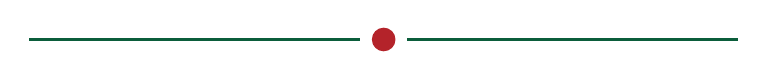
\begin{tikzpicture}
  \draw[Forest,line width=1.2pt] (0,0)--(4.2,0);
  \fill[SignalRed] (4.5,0) circle (1.5mm);
  \draw[Forest,line width=1.2pt] (4.8,0)--(9,0);
\end{tikzpicture}\\[3mm]
{\sffamily\bfseries\color{Forest}AIRGESTURE STUDIO}\\
{\small\color{Slate}Draw naturally. Interact locally.}
\end{center}

\end{document}
